
%(BEGIN_QUESTION)
% Copyright 2006, Tony R. Kuphaldt, released under the Creative Commons Attribution License (v 1.0)
% This means you may do almost anything with this work of mine, so long as you give me proper credit

Følgende lagertank inneholder en væske med tetthet 57.5 lb/ft$^{3}$.  En pneumatisk trykktransmitter i bunnen av tanken beregner væskenivå fra hydrostatisk trykk (head).  Bestem kalibreringsområdet for transmitteren slik at tanknivåområdet (0 til 30 fot) oversettes korrekt til et utgangssignal på 3 til 15 PSI.  Oppgi transmitterens kalibreringsområde i PSI.

$$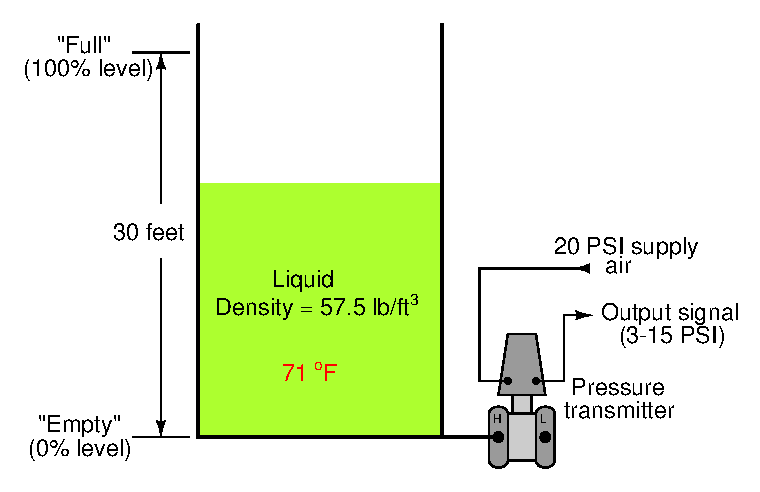
\includegraphics[width=15.5cm]{i00244x01.eps}$$

Bestem deretter følgende (forutsatt at transmitteren er korrekt kalibrert for applikasjonen):

\begin{itemize}
\item{} Transmitterens utgangssignal (PSI) ved 19 fot nivå
\item{} Væskenivå ved 12.4 PSI utgangssignal
\end{itemize}

\underbar{file i00244}
%(END_QUESTION)





%(BEGIN_ANSWER)

Nedre måleverdi (LRV): 0 PSI innsignal = 3 PSI utsignal

\vskip 10pt

Øvre måleverdi (URV): 11.98 PSI innsignal = 15 PSI utsignal

\vskip 10pt

\begin{itemize}
\item{} Transmitterutgang (PSI) ved 19 fot nivå = 10.6 PSI
\item{} Væskenivå ved 12.4 PSI utsignal = 23.5 fot
\end{itemize}

\vskip 10pt

Væsketemperaturen 71 $^{o}$F er overflødig informasjon, inkludert for å utfordre studentene til å avgjøre om informasjon er relevant for en bestemt oppgave.  Væsketemperatur er relevant for nivåinstrumentering fordi temperaturendringer kan endre væsketetthet, og dermed forholdet mellom væskehøyde og hydrostatisk trykk.  Men siden væsketettheten allerede er oppgitt her, er temperaturen irrelevant.

%(END_ANSWER)





%(BEGIN_NOTES)

%INDEX% Measurement, level: hydrostatic pressure

%(END_NOTES)
